\documentclass[a4paper,10pt,onecolumn,oneside,titlepage]{article}

\usepackage[utf8]{inputenc}
\usepackage[spanish]{babel}
\usepackage{graphicx}
\usepackage[left=2cm,right=2cm,top=2cm]{geometry}
\usepackage{float}
\usepackage{rotating}
\usepackage{color}
\usepackage{xcolor}
\usepackage{listings}
\usepackage{caption}
%\usepackage{lscape}

\renewcommand{\baselinestretch}{1.5}
\addtolength{\parindent}{0pt}
\addtolength{\parskip}{\baselineskip}
\bibliographystyle{ieeetr}

\lstset{
% general command to set parameter(s)
basicstyle=\ttfamily, % print whole listing small
keywordstyle=\color{black}\bfseries\underbar, % underlined bold black keywords
identifierstyle=, % nothing happens
commentstyle=\color{white}, % white comments
stringstyle=\ttfamily, % typewriter type for strings
showstringspaces=false % no special string spaces
}

\title{Memoria Final - Arquitecturas Orientadas a la Integración}
\author{Ignacio Robledo Rosell \\
				g990406}
\date{31 de Agosto de 2012}

\includeonly{
	introduccion
%	,
%	ficheroDWG,
%	herramientas,
%	plugin,
%	alcance,
%	desarrollos,
%	pruebas,
%	lineasFuturas,
%	ap1-ejemploUso,
%	ap2-ejemploSalida
}

\begin{document}

\maketitle

\tableofcontents

\section{Introducción.}

Tal y como se menciona en \cite{reusing-silicon}, en los últimos diez años se ha visto un crecimiento sin 
precedentes en el número de dispositivos electrónicos destinados al consumidor final. La gran mayoría de estos dispositivos llevan incorporados microchips. En el cuadro siguiente puede verse la evolución de la facturación de las empresas de materiales semiconductores en el mundo, con crecimientos por encima del 200\% en los últimos 20 años y por encima del 40\% en la última década:

\begin{figure}[H]
\begin{center}
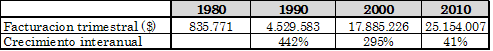
\includegraphics[width=0.8\textwidth]{img/estadisticas_chips}
\caption{Facturación trimestral de empresas de materiales semiconductores en el mundo.}
\end{center}
\end{figure}

Estas estadísticas son publicadas anualmente por la SIA \cite{SIA} (Asociación de la Industria de Semiconductores), que ellos mismos resaltan que representan al 66\% de las compañías de semiconductores del mundo. Por tanto, pueden tomarse, como una muestra representativa de la evolución que sufrido el sector en los últimos 30 años y la dimensión en necesidades de producción del mismo.

Este crecimiento supone un ingente coste económico dado que producir el volumen necesario de microchips y otros componentes requiere una gran cantidad de energía. Aproximadamente se necesitan 600 kilogramos de combustibles fósiles para producir 1 kilogramo de material semiconductor \cite{reusing-silicon}. El coste de la energía se ha incrementado notablemente en los últimos años, con un incremento cercano al 40\% en los últimos 15 años y con una continuada tendencia alcista. A continuación se muestra una gráfica con la evolución del coste medio por kWh en los 15 principales países de la Unión Europea (información proporcionada por Eurostat \cite{eurostat1}):

\begin{figure}[H]
\begin{center}
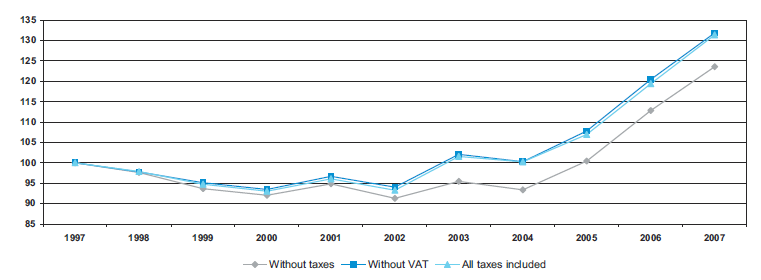
\includegraphics[width=0.8\textwidth]{img/precio_electricidad_industrial}
\caption{Evolución del coste medio de la energía industrial en los 15 principales países de la UE.}
\end{center}
\end{figure}

Otro coste añadido es el medioambiental dado el alto volumen de residuos que se generan al desechar todos estos dispositivos, incluyendo algunos residuos muy contaminantes y muy peligrosos para el medio ambiente.

Por todo ello, en el informe \cite{reusing-silicon} se esboza un planteamiento para reciclar y reutilizar todos estos microchips y componentes semiconductores para la elaboración de nuevos dispositivos y de esta manera:

\begin{itemize}

\item{Reducir la cantidad de energía consumida por la industria de los semiconductores, dado que que el reciclaje de los microchips, puede realizarse con una ínfima parte de la energía empleada en la elaboración de nuevos componentes.}

\item{Reducir los costes soportados por esta industria.}

\item{Reducir la carga medioambiental producida por esta industria, reduciendo el volumen de desechos.}

\end{itemize}.

Los positivos efectos de esta estrategia de reciclaje y reutilización se ven adicionalmente soportados por el hecho de que los microchips y demás componentes actualmente se están infrautilizando muy por debajo del tiempo de vida medio esperado para cada uno de estos componentes (siempre según \cite{reusing-silicon}).

A lo largo de las siguientes secciones de este artículo trataremos de obtener una visión global de en que grado y como esta estrategia de reciclaje y reutilización se ha trasladado al mundo real.
%\include{ficheroDWG}
%\include{herramientas}
%\include{plugin}
%\include{alcance}
%\include{desarrollos}
%\include{pruebas}
%\include{lineasFuturas}
%\include{ap1-ejemploUso}
%\include{ap2-ejemploSalida}

\newpage \bibliography{references}
\newpage \listoffigures
%\listoftables

\end{document}
